\documentclass[a4paper,twosided,12pt,DIV12]{scrartcl}
%
% all the local settings defined in /localsettings.sty
\usepackage{localsettings}
\usepackage{customsymbols}
%
% lazyeqn - math symbols
% Uncomment if you have chosen to clone it to your project
\usepackage{./lazyeqn/lazyeqn}
\addtokomafont{disposition}{\rmfamily}
%
\usepackage{scalefnt}

\newcommand\smallerr[2][0.85]{{\scalefont{#1}#2}}

\newcommand\ilabel[1]{I\smallerr{#1}}
% \usepackage{accents}

% \newcommand\ub[1]{%
%   \underaccent{\bar}{#1}}

% \makeatletter
% \def\ub#1{\underline{\sbox\tw@{$#1$}\dp\tw@\z@\box\tw@}}
% \makeatother

\DeclareMathOperator{\ivt}{ivt}
\DeclareMathOperator{\idxop}{idx}
\DeclareMathOperator{\per}{per}
\DeclareMathOperator{\rank}{rank}
\DeclareMathOperator{\ifop}{if}
\DeclareMathOperator{\invop}{inv}

% \makeatletter
% \newcommand{\idxop}{\mathop{\operator@font idx}}
% \newcommand{\per}{\mathop{\operator@font per}}
% % \newcommand{\ivt}{\mathop{\operator@font ivt}}
% \newcommand{\rank}{\mathop{\operator@font rank}}
% \newcommand{\ifop}{\mathop{\operator@font if}}
% \newcommand{\invop}{\mathop{\operator@font inv}}
% \makeatother

\newcommand{\veps}{\vareps}

% \def\ub#1{\underline{\smash{#1}}}
\def\ub#1{\underline{#1}}

% \newcommand{\idx}[1]{#1_1 #1_2 \dotsm #1_N}
% \newcommand{\idxu}[1]{\ub{#1}_1 \ub{#1}_2 \dotsm \ub{#1}_N}
% \newcommand{\idxn}[2]{#1_1 #1_2 \dotsm #1_{#2}}
% \newcommand{\idxnu}[2]{\ub{\idxn{#1}{#2}}}

\newcommand{\idx}[1]{#1_1 \dotsm #1_N}
\newcommand{\idxu}[1]{\ub{#1}_1 \dotsm \ub{#1}_N}
\newcommand{\idxn}[2]{#1_1 \dotsm #1_{#2}}
\newcommand{\idxnu}[2]{\ub{\idxn{#1}{#2}}}

%
\frenchspacing
%
% \title{Array Calculus}
\title{Composites Modeling WS2014--2015 Assignment}
\author{Huseyin Onur Solmaz -- Matr.2868402}
\date{}
%



\begin{document}
\maketitle
\tableofcontents

\section{Estimation of Material Constants (Task 1)}

\textit{The following tables give typical mechanical data for T300 carbon-fiber and
Hexcel 8551-7 epoxy resin.}

\begin{table}[H]
  \centering
  \begin{minipage}{0.45\textwidth}
    \footnotesize
  \begin{tabular}{p{0.7\textwidth}p{0.2\textwidth}}
    \toprule
    Fiber type & T300\\
    Longitudinal modulus $E_{1}$ (GPa) & 231\\
    Transverse modulus $E_{12}$ (GPa) & 15\\
    Transverse modulus $E_{13}$ (GPa) & 15\\
    In-plane shear modulus $G_{f12}$ (GPa) & 15\\
    Major Poisson's ratio $\nu_{f12}$ & 0.2\\
    Major Poisson's ratio $\nu_{f13}$ & 0.2\\
    Transverse shear modulus $G_{f23}$ (GPa) & 7\\
    Longitudinal tensile strength $X_{f1T}$ (MPa) & 2500\\
    Longitudinal compressive strength $X_{f1C}$ (MPa) & 2000\\
    Longitudinal tensile failure strain $\veps_{f1T}$ (\%) & 1.086\\
    Longitudinal compressive failure strain $\veps_{f1C}$ (\%) & 0.869\\
    \bottomrule
  \end{tabular}
  \end{minipage}
  \begin{minipage}{0.45\textwidth}
    \footnotesize
  \begin{tabular}{p{0.7\textwidth}p{0.2\textwidth}}
    \toprule
    Matrix type & 8551-7 epoxy\\
    Elastic modulus $E_{m}$ (GPa) & 4.08\\
    Elastic shear modulus $G_{m}$ (GPa) & 1.478\\
    Elastic Poisson's ratio $\nu_{m}$ (GPa) & 0.38\\
    Tensile strength $Y_{mT}$ (MPa) & 99\\
    Compressive strength $Y_{mC}$ (MPa) & 130\\
    Shear strength $S_{m}$ (MPa) & 57\\
    Tensile failure strain $\veps_{mT}$ (\%) & 4.4\\
    Compressive failure strain $\veps_{mC}$ (\%) & 9\\
    Shear failure strain $\gamma_{m}$ (\%) & 5.1\\
    \bottomrule
  \end{tabular}
  \end{minipage}
  \caption{Material parameters for the carbon-fibers (left) and epoxy resin
    matrix (right).}
\end{table}
\subsection{Estimation (Part a)}

\textit{Use necessary micro-mechanics formulae to estimate elastic modulus
  ($E_{1}$, $E_{2}$,
$G_{12}$), Poisson's ratios ($\nu_{12}$ and $\nu_{21}$) and failure properties for maximum stresses
($F_{1T}$, $F_{1C}$, $F_{2T}$, $F_{2C}$ and $F_{12}=F_{6}$) assuming the composite is unidirectional
with \textbf{a fiber volume ratio of 50\%}}
\subsubsection{Elastic and Shear Moduli}
%
$V_f$, the fiber volume fraction  is given to be $0.5$. The longitudinal
modulus $E_1$ for the \emph{Representative Volume Element} RVE is calculated as
%
\begin{equation}
  E_1 = E_fV_f + E_m (1-V_f)
\end{equation}
%
where $E_f$ and $E_m$ are the longitudinal moduli of the fibers and matrix
respectively. Using the formula, $E_1$ = \SI{117.54}{GPa}.
%
\\The inverse mixture relation is used for the transverse modulus $E_2$
%
\begin{equation}
  \frac{1}{E_2} = \frac{V_f}{E_{2f}} + \frac{V_m}{E_m}
  \eqor
  E_2 = \frac{E_{2f} E_m}{V_mE_{2f}+V_fE_m}
\end{equation}
%
where $E_{2f}$ is the transverse modulus of the fibers, and $V_m$ is the folume
fraction of the matrix. Using the formula, $E_2$ = \SI{6.415}{GPa}.
\\Similarly, the shear modulus is calculated as
%
\begin{equation}
  \frac{1}{G_{12}} = \frac{V_f}{G_{f12}} + \frac{V_m}{G_m}
  \eqor
  G_{12} = \frac{G_{f12} G_m}{V_mG_{f12}+V_fG_m}
\end{equation}
%
where $G_{f12}$ and $G_m$ are the shear moduli of the fibers and the matrix
respectively. Using the formula, $G_{12}$ = \SI{2.691}{GPa}.
%
\subsubsection{Hopkins-Chamis Model}
%
The Hopkins-Chamis model can be used to make a better estimate of $E_2$ and
$G_{12}$. It goes for $E_2$
%
\begin{equation}
  E_{2} = E_m\sbr{\sbr{1-\sqrt{V_f}}+\frac{\sqrt{V_f}}{1-\sqrt{V_f}\sbr{1-\frac{E_m}{E_{f2}}}}}
\end{equation}
%
yielding $E_2$ = \SI{7.141}{GPa}. Similarly $G_{12}$ = \SI{3.315}{GPa}.
%
These values will be used for all calculations.
%
%
\subsubsection{Poisson's Ratios}
%
Major and minor Poisson's ratios will be calculated following the same
principle, using direct and inverse mixture relations
%
\begin{gather}
  \nu_{12} = \nu_{f12} V_f + \nu_m V_m\\
  \frac{1}{\nu_{21}} = \frac{V_f}{\nu_{f21}} + \frac{V_m}{\nu_m}
  \eqor
  \nu_{21} = \frac{\nu_{f21} \nu_m}{V_m\nu_{f21}+V_f\nu_m}
\end{gather}
%
where $\nu_{12}$, $\nu_{21}$ and $\nu_m$ are the major and minor Poisson's
ratios and the Poisson ratio of the matrix respectively. Using the formulas,
$\nu_{12}$ = 0.290, $\nu_{21}$ = 0.262.
%
\subsubsection{Maximum Stresses}
\textbf{The failure stress at longitudinal tension} is calculated using the direct relation
%
\begin{equation}
  F_{1t} = \sigma_f V_f  + \sigma_m^{*} (1-V_f)
\end{equation}
where $\sigma_f$ is the longitudinal tensile strength of the
fibers and $\sigma_m^{*}$ is matrix stress at failure. The last one is
calculated as
\begin{equation}
  \sigma_m^{*} \approx \sigma_f \frac{E_m}{E_f}
\end{equation}
Using the formulas, $\sigma_m^{*}$ = \SI{44.156}{MPa} $F_{1t}$ = \SI{1272.1}{MPa}.
%
\\\textbf{The failure stress at transverse tension} is calculated as
%
\begin{equation}
  F_{2t} = E_{2} \veps_{2t\textsf{ult}}
\end{equation}
%
where $\veps_{2t\textsf{ult}}$ is the ultimate transverse strain at tension
%
\begin{equation}
  \veps_{2t\textsf{ult}} = \frac{\veps_{m\textsf{ult}}}{F}
\end{equation}
%
where $F$ is the \emph{stress concentration factor}
%
\begin{equation}
  F = \frac{\veps_m}{\veps_c} = \frac{1}{\frac{d}{s}\sbr{\frac{E_m}{E_f}-1}+1}
\end{equation}
%
Here $\frac{d}{s}$ is related to spatial configuration, and is equal to
$\sqrt{\frac{2}{\pi}}$. From this $F$ = 2.386.
$\veps_{m\textsf{ult}}$ is derived from the simple
relation
%
\begin{equation}
  Y_{mT} = E_m \veps_{m\textsf{ult}}
\end{equation}
and leads to $\veps_{m\textsf{ult}}$ = \num{24.265e-3} therefore $\veps_{2t\textsf{ult}}=$
\num{10.17e-3}. $F_{2t}$ is finally found out to be \SI{72.624}{MPa} using the
moduli obtained from Hopkins-Chamis model.
%
\\\textbf{The failure stress at longitudinal compression} is calculated for 3
different failure cases
\begin{enumerate}
\item For fiber micro-buckling,
  \begin{equation}
    F_{1c} = \frac{G_m}{1-V_f}
  \end{equation}
  and equals \SI{2956}{MPa}.

\item Transverse tensile rupture due to Poisson's effect
%
  \begin{equation}
    F_{1c} = \frac{E_{1}\veps_{2t\textsf{ult}}}{\nu_{12}}
  \end{equation}
  Using previously calculated values, \SI{4122}{MPa}.

\item Shear failure without buckling
%
  \begin{equation}
    F_{1c} =  2\rbr{\tau_{f\textsf{ult}}V_f + \tau_{m\textsf{ult}}V_m}
  \end{equation}
  where
    $\tau_{f\textsf{ult}} = \frac{\sigma_{\textsf{ult}}}{2}$ = \SI{1000}{MPa}
    and $\tau_{m\textsf{ult}}$ = \SI{57}{MPa} from given values. This yields
    \SI{1057}{MPa} for this case.
\end{enumerate}
%
%
\textbf{The failure stress at transverse compression} is calculated in the same
manner as transverse tension
%
\begin{equation}
  F_{2c} = E_{2} \veps_{2c\textsf{ult}}
\end{equation}
%
where $\veps_{2c\textsf{ult}}$ is the
%
\begin{equation}
  \veps_{2c\textsf{ult}} = \frac{\veps_{mc\textsf{ult}}}{F}
\end{equation}
%
where $F$ is the same stress concentration factor defined before and again
equals 2.386.
$\veps_{mc\textsf{ult}}$ is calculated similarly
%
\begin{equation}
  Y_{mC} = E_m \veps_{mc\textsf{ult}}
\end{equation}
and leads to $\veps_{mc\textsf{ult}}$ = \num{31.863e-3} therefore $\veps_{2c\textsf{ult}}=$
\num{13.354e-3}. $F_{2c}$ is finally found out to be \SI{95.361}{MPa}.
%
\\\textbf{The in-plane shear strength} is calculated as
%
\begin{equation}
  F_6 = F_{12} = G_{12}\gamma_{12}
\end{equation}
%
where
%
\begin{equation}
  \gamma_{12} = \frac{\gamma_{m\textsf{ult}12}}{F_s}
\end{equation}
%
where $\gamma_{m\textsf{ult}12}$ can be found from the relation
%
\begin{equation}
  S_m = G_m \gamma_{m\textsf{ult}12}
\end{equation}
%
and $F_s$ is the shear stress concentration factor defined as
%
\begin{equation}
  F_s = \frac{\gamma_{m12}}{\gamma_{c12}} = \frac{1}{\frac{d}{s}\sbr{\frac{E_{m12}}{E_{f12}}-1}+1}
\end{equation}
%
again, $\frac{d}{s}=\sqrt{\frac{2}{\pi}}$ and $F_s$ = \num{3.56}.
$\gamma_{m\textsf{ult}12}$ = \num{38.566e-3} and $\gamma_{12}$ =
\num{10.833e-3}. Hence $F_6$ = \SI{33.916}{MPa}.

\begin{table}[htbp]
  \centering
  \begin{tabular}{lll}
    \toprule
    Composite longitudinal modulus & $E_1$ & \SI{117.54}{GPa}\\
    Composite transverse modulus & $E_2$ & \SI{7.141}{GPa}\\
    Composite shear modulus & $G_{12}$ & \SI{3.315}{GPa}\\
    Composite major Poisson's ratio &$\nu_{12}$ & \num{0.290}\\
    Composite minor Poisson's ratio &$\nu_{21}$ & \num{0.262}\\
    Composite longitudinal tension strength & $F_{1t}$ & \SI{1272.1}{MPa}\\
    Composite transverse tension strength & $F_{2t}$ & \SI{72.624}{MPa}\\
    Composite longitudinal compression strength, buckling & $F_{1c}$ & \SI{2956}{MPa}\\
    Composite longitudinal compression strength, rupture  & $F_{1c}$ & \SI{4122}{MPa}\\
    Composite longitudinal compression strength, shear failure & $F_{1c}$ & \SI{1057}{MPa}\\
    Composite transverse compression strength & $F_{2c}$ & \SI{95.361}{MPa}\\
    Composite in-plane shear strength & $F_{12}$ & \SI{33.916}{MPa}\\
    \bottomrule
  \end{tabular}
  \caption{Results of micromechanics calculations}
\end{table}

\subsection{Discussion (Part b)}

\textit{Briefly discuss the limitations of micro-mechanics to predict mechanical
properties, especially failure properties.}

\section{}
\textit{This uni-directional composite is used for a simple square flat plate as shown
below having a length of 400mm and with 300mm. Eight plies having a symmetric
lay-up [0/90/+45/-45]s are used. Assume the ply thickness is 0.25mm and the
0\degree fiber direction is in the plate length (x) direction.
\\The composite plate has a line load as shown and is simply supported at both
ends in the width direction.}

\begin{center}
  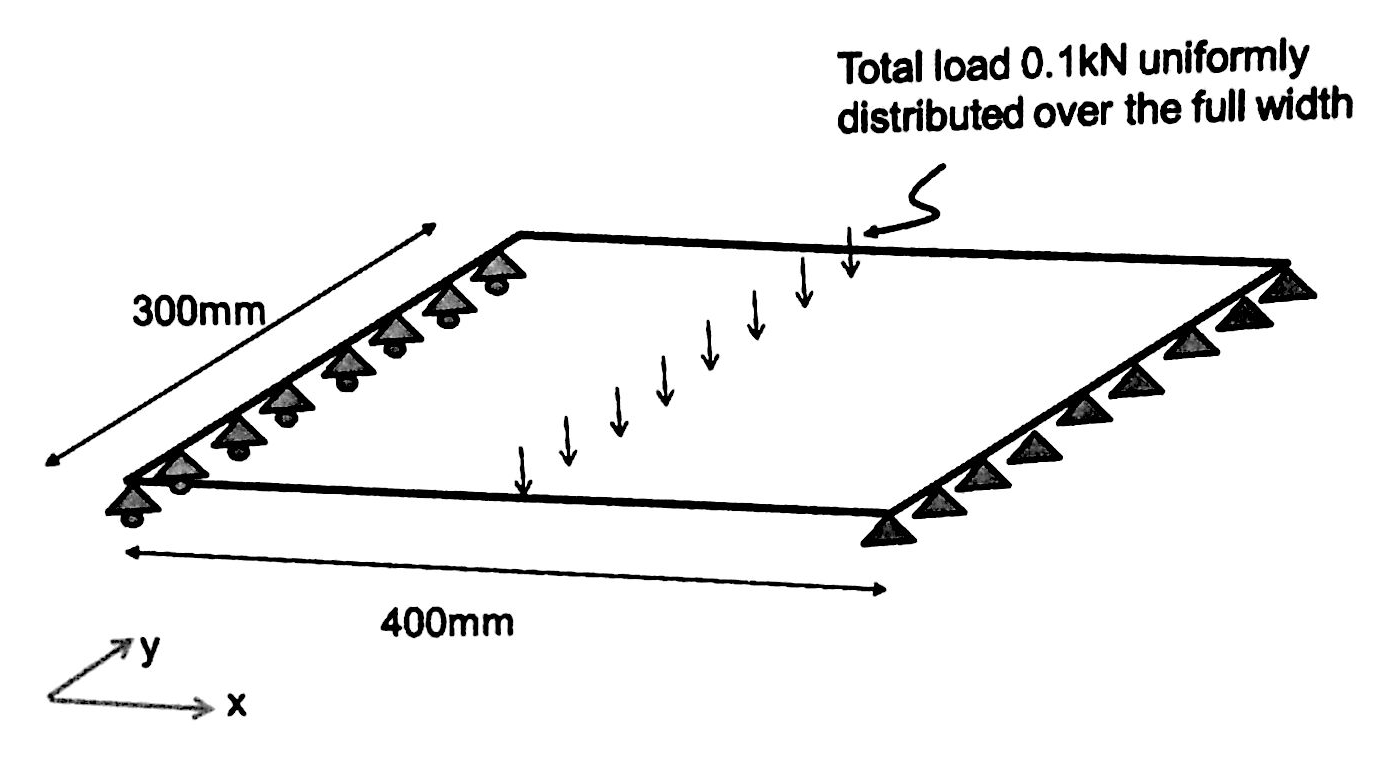
\includegraphics[width=0.7\textwidth]{fig1.png}
\end{center}

\subsection{}

\textit{Use laminate analysis to compute the relevant laminate stiffnesses and classical
beam bending formulae to estimate maximum deflection at the center of the
plate.}

\subsection{}

\textit{Use laminate analysis and the failure data from question 1, to estimate the
first and last ply failure loads.}

\section{}

\textit{Create a Finite Element model of the above problem having identical
boundary conditions, loadings and material properties.
\\Perform an implicit Finite Element analysis and compute the central
deflection. Compare results with the previous classical solution using laminate
analysis.}

\section{}

\textit{Modify the above finite element model to include two geometric stiffeners (so
called Beads or Sikkens). Choose a suitable spacing for the sickens with each
one having approximate dimensions of 250mm length and 30mm with (15mm height).
Note a useful option exists in Visual Mesh for this operation (2D > Bead on 2D mesh).
The plate with Sikkens has identical loading (line load across the center) and
boundary conditions identical to question 2.}

\begin{center}
  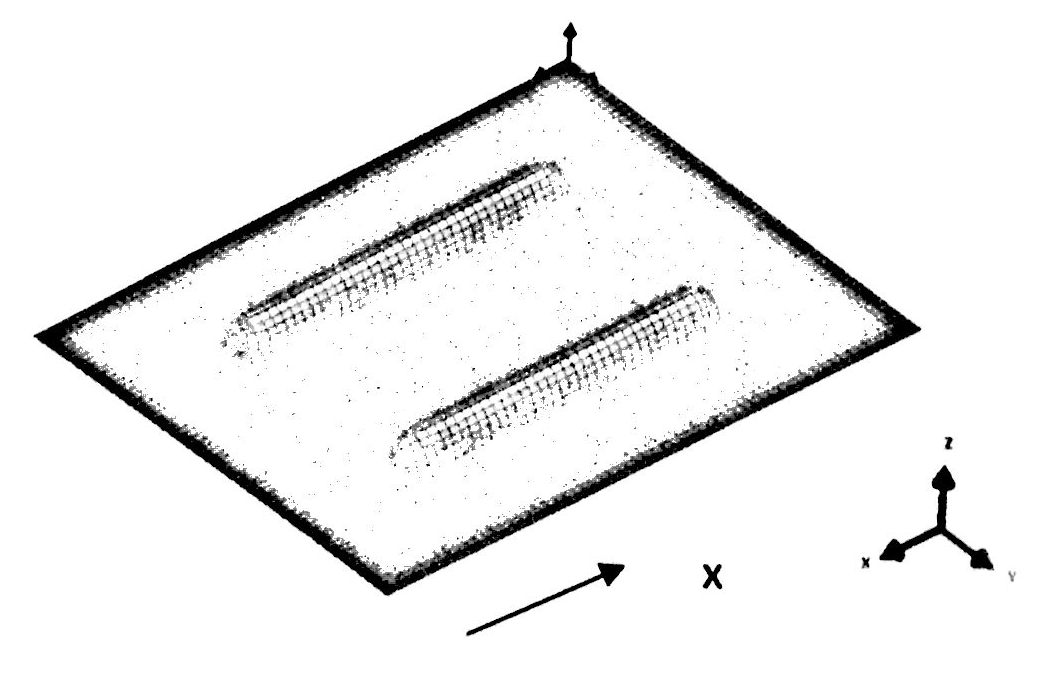
\includegraphics[width=0.7\textwidth]{fig2.png}
\end{center}

\textit{Use the ILAY=1 option to define the laminate, which has the same materials,
lay-up orientations and ply thicknesses as used in questions 2 and 3. Define
Auxiliary 26 to get the failure load indicator for all plies (done in the
material cards). For the output contours to work properly, you will need to use
the ILAY=1 option and also visualize results from the .erfh5 file (for erf5 file
output set ERFKEY=3 in the OCTRL control card).}

\textit{Perform an implicit failure analysis of the plate with Sikkens and compute
\begin{enumerate}
\item The maximum deflection.
\item The failure load using a maximum stress criterion and the composite
  failure data determined from question 1.
\item From the contour results for ``Ply Failure Criteria'' estimate the
  necessary applied load to just cause first ply failure of the structure.
\end{enumerate}}

\section{}
%
\textit{Perform a PAM-RTM infusion simulation of the Plate with Sikkens.
\\Beware that PAM-RTM uses only triangular shell elements and the units should
be in meters, if you want to be consistent with default data provided in
PAM-RTM. Both element type (option MESH > TRANSFORM > SPLIT QUADS...) and units
(option MESH > TRANSFORM > SCALE...) can be converted in PAM-RTM, or in Visual
Mesh with similar options.
\\Assume the resin inlet is as shown below. Use pressure injection with 1 bar
difference between inlet and outlet. Assume the infusion is isothermal at room
temperature and the fabric has isotropic permeability throughout.}
%
\begin{table}[H]
  \centering
  \begin{tabular}{ll}
    \toprule
    Thickness of composite & 2 mm\\
    Resin viscosity at 23\degree C & 0.3 Pa sec \\
    Assume PAM-RTM standard fabric with porosity & 0.5 \\
    Fabric permeability & \num{1e-10} m\textsuperscript{2}\\
    \bottomrule
  \end{tabular}
  \caption{Infusion and other data}
\end{table}
%
\begin{center}
  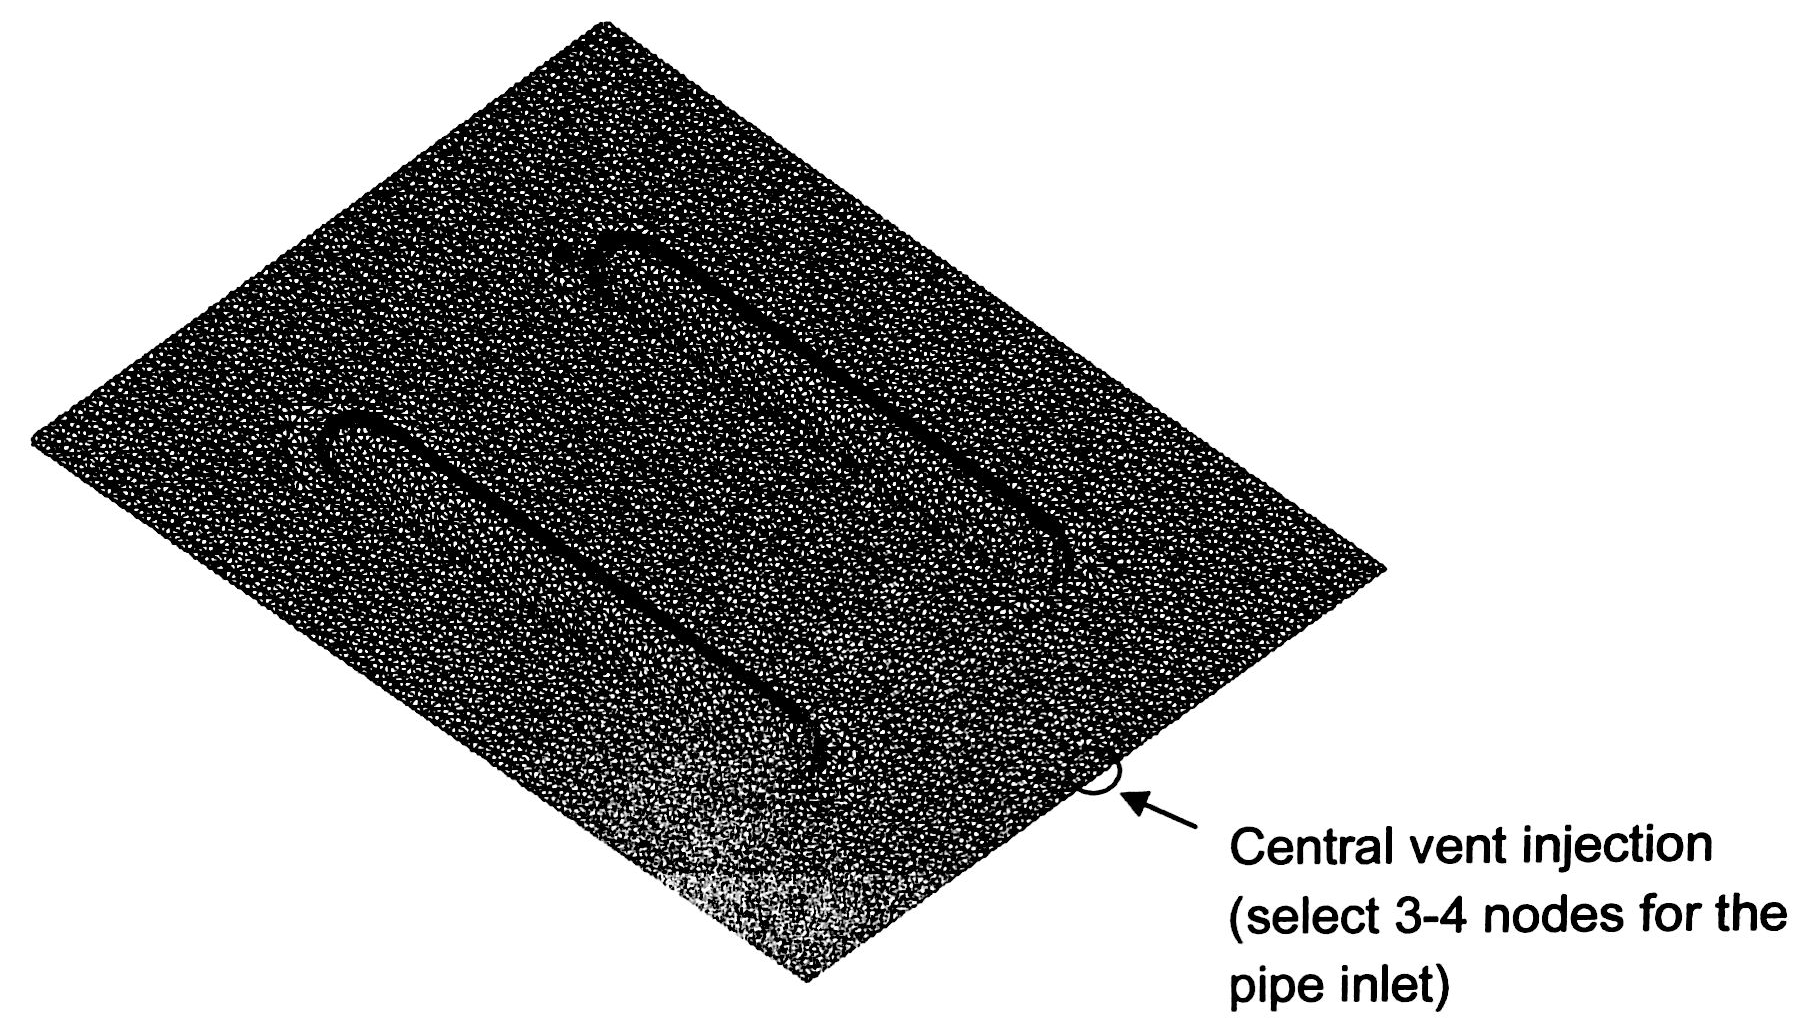
\includegraphics[width=0.7\textwidth]{fig3.png}
\end{center}
%
\textit{Perform an RTM type analysis and estimate:
%
\begin{enumerate}
\item The time for infusion and suitable positions for the outlet vents.
\item If the resin is known to gel after 30 minutes, is the infusion likely to
  be successful?
\item Propose and try an alternative infusion strategy with a view to speeding
  up the infusion time and having a good infusion. Where should the outlet vents
  be placed for your chosen setup?
\end{enumerate}}


\end{document}
%
